\subsection{Overview}Let $\mathcal{D} = \{(\mathbf{X}_n, \mathbf{Y}_n)\}_{n=1}^{N}$ denote the training dataset,
where $N$ is the total number of training images, $\mathbf{X}_n \in \mathbb{R}^{H \times W \times C}$ is the $n$-th input image ($C$ is the number of channels),
and $\mathbf{Y}_n = \{y_{n,i,j}\}_{i,j} \in \mathbb{R}^{H \times W}$ is the corresponding ground truth mask.
In uncertainty estimation using MC Dropout, $T$ stochastic inferences are performed for each image.
We denote the predicted probability map in the $t$-th inference ($t \in \{1, \ldots, T\}$) as $\hat{\mathbf{Y}}_n^{(t)} = \{\hat{y}_{n,i,j}^{(t)}\}_{i,j}$.

Fig.~\ref{method} illustrates the overview of the proposed method. The design of this method is primarily based on the following two perspectives.
First, the difficulty assessment for training samples is dynamically updated during the learning process.
Since image difficulty is not absolute but relative, changing with the model's training progress,
sequentially re-evaluating difficulty based on the current state of the model allows learning to focus on images where the model currently lacks confidence.
Second, epistemic uncertainty is suitable as a quantitative metric for difficulty. Since epistemic uncertainty stems from the model's lack of knowledge,'' 
it directly reflects unlearned patterns or regions where the model is hesitant. Therefore, it allows for the appropriate quantification of how unconfident the model is,''
which can be improved through learning, without being affected by noise.

In the proposed method, MC Dropout is used every $\tau$ epochs during training to perform multiple inferences for each image,
and uncertainty is quantified from the variance of the predictions.This uncertainty information reflects the degree of the model's lack of confidence
in the segmentation of that image.Subsequently, this uncertainty information is aggregated on a per-image basis to dynamically control the shape of the PolyDice Loss,
assigning steeper gradients to difficult images and gentler gradients to easy images.By applying the updated $\epsilon$ to the training in the next $\tau$ epochs,
we realize adaptive learning that dynamically changes the optimization weighting according to the progress of learning.

\clearpage

\begin{figure}
    \includegraphics[width=\columnwidth]{figure/method.pdf}
    \caption{Overview of the proposed adaptive learning framework.The process consists of two phases: uncertainty estimation and adaptive training. Every $\tau$ epochs,
    the model evaluates image difficulty using MC Dropout and updates the loss shape parameter $\epsilon$. This dynamic control assigns steeper gradients to harder samples, enabling difficulty-aware optimization.}
    \label{method}
\end{figure}

\clearpage

\subsection{Quantification of Image Difficulty Based on Uncertainty}
\subsubsection{MC Dropout Inference During Training}
In the proposed method, the learning process is divided into two phases:
an initial training phase and an adaptive training phase.
The period from epoch $1$ to $E_0 - 1$ is defined as the initial training phase,
where training is performed with the loss shape parameter $\epsilon$ fixed at $0$.
The reason for establishing this period is that the feature representation of the model is immature in the early stages of learning,
and uncertainty at this stage depends more on the model's initialization than on the intrinsic difficulty of the image.
$E_0$ is set as the number of epochs sufficient for the model to acquire basic segmentation capabilities.
In the adaptive training phase ($e \geq E_0$), the re-evaluation of uncertainty and the update of $\epsilon$ are performed every period $\tau$.
That is, the update is executed before the start of learning for epochs satisfying $e \in \{E_0, E_0+\tau, E_0+2\tau, \ldots\}$.
During the update, the model parameters $\mathbf{W}$ at that point are fixed, and $T$ stochastic inferences are performed for each image
$\mathbf{X}_n$ in the training data with a Dropout rate $p \in (0,1)$.Let the obtained set of predictions be 
$\{\hat{\mathbf{Y}}_n ^ {(t)}\}_{t=1}^{T}$:
\begin{equation}
    \hat{\mathbf{Y}}_n ^ {(t)} = f_{\mathbf{W}}(\mathbf{X}_n; \mathbf{z}^{(t)}), \quad \mathbf{z}^{(t)} \sim \text{Bernoulli}(1-p)
\end{equation}
Here, $\mathbf{z}^{(t)}$ is the Dropout mask for the $t$-th inference, and $\hat{\mathbf{Y}}_n ^ {(t)}$ is the resulting predicted probability map.
The model's epistemic uncertainty is quantified from the variance of predictions obtained through this stochastic inference.

\subsubsection{Calculation of Pixel-wise Uncertainty Metrics}For the $T$ predicted images obtained by MC Dropout,
we calculate the Mutual Information $I_{n, i, j}$, which can directly capture epistemic uncertainty, as a pixel-wise uncertainty metric.
\begin{equation}
    I_{n, i, j} = \underbrace{H\left( \frac{1}{T} \sum_{t=1}^{T} \hat{y}_{n, i,j}^{(t)} \right)}_{\text{Entropy of Mean}} - \underbrace{\frac{1}{T} \sum_{t=1}^{T} H\left( \hat{y}_{n, i,j}^{(t)} \right)}_{\text{Mean of Entropy}}
\end{equation}
Here, $H(p)$ is the binary entropy function for binary classification, defined as follows:
\begin{equation}
    H(p) = -p \log p - (1-p) \log (1-p)
\end{equation}
Mutual Information is widely used as a metric to evaluate the uncertainty accompanying model predictions and to isolate its underlying factors.
It quantifies epistemic uncertainty by subtracting the expected entropy (the mean of the entropy of individual inferences),
which indicates aleatoric uncertainty derived from data-inherent noise and ambiguity, from the predictive entropy,
which is the uncertainty of the predictive distribution after averaging $T$ inference results (indicating uncertainty from both data and model).
High values in a region suggest that the model has not sufficiently learned that area.

\subsubsection{Aggregation to Image Level}
The mean value of the pixel-wise mutual information, after outlier removal, is quantified as the difficulty metric for the entire image.
In medical image segmentation, there is an extreme class imbalance where background regions occupy the majority of the image,
while the lesion areas of interest are extremely small. Background regions are generally easy to infer,
and their uncertainty tends to take extremely low values. Therefore, if the average uncertainty is calculated over the entire image,
the low values from the massive number of background pixels may dominate the overall difficulty metric, failing to properly quantify the local difficulty of the lesion that should be captured.
Therefore, to sensitively reflect the difficulty of lesion detection, the proposed method calculates the average mutual information restricted to the lesion region in the ground truth mask.
Let $\Omega_n$ be the entire image domain, and $\mathcal{P}_n = \{(i,j) \in \Omega \mid y_{i,j} = 1\}$ be the set of pixels in the positive region of the ground truth mask.
Here, the calculated mutual information may contain sporadic noise or extreme outliers, which can destabilize the quantification of the difficulty metric.
Therefore, prior to calculating the score, statistical outlier removal is performed. Specifically,
let $\mu_{\mathcal{P}_n}$ be the mean and $\sigma_{\mathcal{P}_n}$ be the standard deviation of the mutual information within the region $\mathcal{P}_n$.
The valid pixel set $\mathcal{P}_n'$ is defined as follows:
\begin{equation}
    \mathcal{P}_n' = \left\{ (i,j) \in \mathcal{P}_n \mid \mu_{\mathcal{P}_n} - 2\sigma_{\mathcal{P}_n} \leq I_{n, i, j} \leq \mu_{\mathcal{P}_n} + 2\sigma_{\mathcal{P}_n} \right\}
\end{equation}
The rationale for adopting $2\sigma_{\mathcal{P}_n}$ as the threshold is based on the concept of statistical confidence intervals.
Assuming the distribution of mutual information approximates a normal distribution, approximately $95\%$ of all data falls within the range of $\pm 2\sigma$ centered on the mean.
Therefore, by rejecting data outside this range, statistically singular extreme values (outliers) are effectively removed, enabling robust difficulty estimation that reflects the main features of the lesion.
Using this valid set $\mathcal{P}_n'$, the difficulty score $D_n$ for the entire image is calculated as:
\begin{equation}
    D_n = \frac{1}{|\mathcal{P}_n'|} \sum_{(i,j) \in \mathcal{P}_n'} I_{n, i,j}
\end{equation}
Here, $|\mathcal{P}_n'|$ represents the number of pixels in the positive region after outlier removal. Note that for images with no positive region, $D_n = 0$.

Next, to determine the relative difficulty of each sample, normalization is performed based on the difficulty score distribution of the entire dataset.
The purpose here is to absorb numerical scale differences between images and evaluate how relatively difficult each image is within the overall distribution.
Given the set of scores $\{D_n\}_{n = 1} ^ N$ for the entire dataset, let $D_q$ be the $q$-th percentile value and $\sigma_D$ be the standard deviation.
The normalized score is calculated as follows:
\begin{equation}
    D_{n} ^ {\text{norm}} = \frac{D_n - D_{q}}{\sigma_D + \delta}
\end{equation}
Here, $\delta > 0$ is a small constant for numerical stability.Subtraction by $D_q$ serves to center the input for the control function described later.
By using the $q$-th percentile instead of the mean of the distribution, the baseline for difficulty can be flexibly set without being affected by outliers,
even in distributions dominated by easy samples.Division by $\sigma_D$ unifies the scale,
serving to adjust the sensitivity of the control function so that it does not depend on the scale of uncertainty specific to each dataset.

\subsection{Adaptive Loss Shape Control}\
subsubsection{Design of the Control Function}
Based on the obtained difficulty metric $D_{n} ^ {\text{norm}}$, the shape parameter $\epsilon$ of the PolyDice-1 Loss is dynamically updated.
We use the following sigmoid-based control function for the update equation.
\begin{equation}
    \epsilon = \epsilon_{\text{min}} + (\epsilon_{\text{max}} - \epsilon_{\text{min}}) \sigma(k \cdot D_{n} ^ {\text{norm}})
\end{equation}
Here, $\sigma(x) = (1 + e^{-x})^{-1}$ is the standard sigmoid function, $k > 0$ is a parameter, and $\epsilon_{\text{min}}, \epsilon_{\text{max}}$ represent the variation range of $\epsilon$.
The reason for adopting the sigmoid function in this method lies in its boundedness and smoothness.Abrupt switching, such as with a step function,
ay compromise training stability,while a linear function may cause the parameter $\epsilon$ to deviate from the appropriate range $[\epsilon_{\text{min}}, \epsilon_{\text{max}}]$.
By using the sigmoid function, it is possible to smoothly transition from low to high difficulty regions while strictly constraining the output value within a predetermined range.
The parameter $k$ controls the response sensitivity of the function; as shown in Fig.~\ref{sigmoid}, a larger value results in a steeper boundary for difficulty judgment,
while a smaller value results in a smoother transition.Through this control, a large $\epsilon$ is assigned to difficult images (large $D_{n} ^ {\text{norm}}$),
making the gradient of the loss function steeper.This implies giving a larger loss value and gradient for the same prediction error,
resulting in the relative strengthening of the learning signal from difficult images.On the other hand, a small $\epsilon$ is assigned to easy images that have already been sufficiently learned,
preventing overfitting while concentrating learning resources on difficult images.The updated $\epsilon$ is applied to training, enabling the model to focus on learning difficult images.

\clearpage

\begin{figure}
    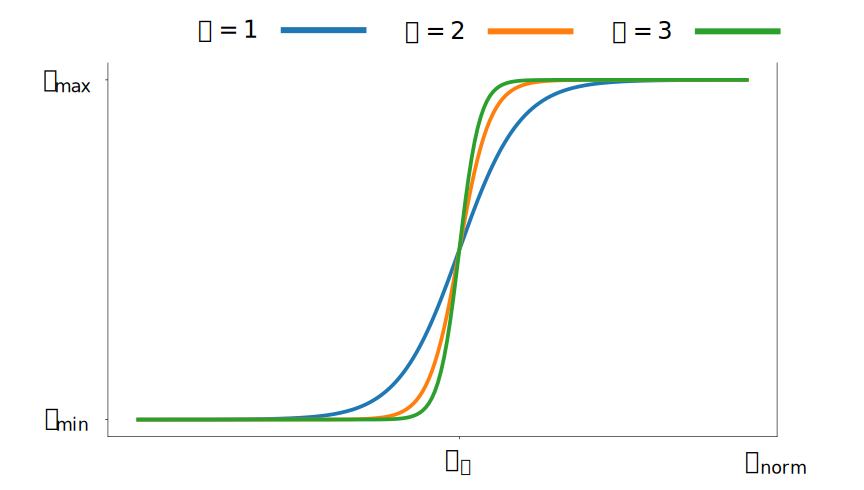
\includegraphics[width=\columnwidth]{figure/sigmoid_sensitivity.pdf}
    \caption{Sigmoid-based control function for loss shape parameter $\epsilon$}
    \label{sigmoid}
\end{figure}

\clearpage

\subsubsection{Learning Algorithm}
Algorithm \ref{alg:proposed_method} presents the detailed algorithm.The learning process consists of two components: adaptive control,
which performs difficulty evaluation and loss parameter updates, and the training phase, which actually updates the model parameters.At the start of training,
the model parameters $\mathbf{W}$ are initialized, and the loss shape parameter $\epsilon$ for all images is initialized to $0$.
In the case where $E_0 > 0$, the period from epoch $1$ to $E_0 - 1$ is the initial training phase, and training is performed with the standard PolyDice-1 Loss fixing $\epsilon=0$.Through this period,
the model acquires the fundamental feature representations necessary for uncertainty estimation.If $E_0 = 0$, adaptive control begins from the first epoch.In the adaptive training phase ($e \geq E_0$),
adaptive control is executed every $\tau$ epochs.Here, following the procedure described in Section 3.2, $\epsilon$ for each image is updated through uncertainty metric estimation via MC Dropout inference,
aggregation to image units, and normalization.Note that during the adaptive control stage, the model parameters $\mathbf{W}$ are fixed,
and only the update of the loss function shape parameter $\epsilon$ is performed.In the subsequent training phase (Epoch $e$),
mini-batch learning is performed using the updated $\epsilon$.Specifically, let $\mathcal{B} \subset \{1, \dots, N\}$ be the set of indices of images constituting a randomly sampled mini-batch.
The objective function $\mathcal{L}$ to be optimized is defined as the average of the PolyDice-1 Loss using the shape parameter $\epsilon_n$ individually assigned to each image $n \in \mathcal{B}$ in the batch, as follows:

\begin{equation}
    \mathcal{L} = \frac{1}{|\mathcal{B}|} \sum_{n \in \mathcal{B}} \mathcal{L}_{\text{PolyDice-1}}(\hat{\mathbf{Y}}_n, \mathbf{Y}_n; \epsilon_n)
\end{equation}

Here, $\mathcal{L}_{\text{PolyDice-1}}(\cdot; \epsilon_n)$ represents the loss function for a single image with parameter $\epsilon_n$ applied.
By applying a different $\epsilon_n$ to each image in the batch in this way, it becomes possible to simultaneously assign steep gradients to images determined to be high difficulty and gentle gradients to low difficulty images.
Finally, the model parameters $\mathbf{W}$ are optimized by gradient descent based on this loss function $\mathcal{L}$.
By repeating this cycle, it becomes possible to focus learning on difficult images according to the model's training progress.

\clearpage

\begin{algorithm}[t]
    \caption{Uncertainty-based Adaptive PolyDice-1 Loss Learning Algorithm}
    \label{alg:proposed_method}
    \begin{algorithmic}[1]
        \small
        \Require Training dataset $\mathcal{D} = \{(\mathbf{X}_n, \mathbf{Y}_n)\}_{n=1}^{N}$
        \Require Model $f_{\mathbf{W}}$, Max epochs $E$
        \Require \textbf{Hyperparameters:} Dropout probability $p$, Start epoch $E_0$, Interval $\tau$, MC iterations $T$, Normalization percentile $q$, Slope $k$, Range $[\epsilon_{\text{min}}, \epsilon_{\text{max}}]$
        
        \State Initialize model parameters $\mathbf{W}$
        \State Initialize loss parameters $\epsilon_n \leftarrow 0$ for all $n \in \{1, \dots, N\}$
        
        \For{$e = 1$ \textbf{to} $E$}
            \If{$e \geq E_0$ \textbf{and} $(e - E_0) \pmod \tau = 0$}
                \State Set model to evaluation mode (enable Dropout)
                
                \For{$n = 1$ \textbf{to} $N$}
                    \For{$t = 1$ \textbf{to} $T$}
                        \State $\hat{\mathbf{Y}}^{(t)} = f_{\mathbf{W}}(\mathbf{X}_n; \mathbf{z}^{(t)}), \quad \mathbf{z}^{(t)} \sim \text{Bernoulli}(1-p)$
                    \EndFor
                    
                    \State Calculate pixel-wise Mutual Information (Eq. 9):
                    \State $I_{n, i,j} = H\left( \frac{1}{T} \sum_{t=1}^{T} \hat{y}_{n, i,j}^{(t)} \right) - \frac{1}{T} \sum_{t=1}^{T} H\left( \hat{y}_{n, i,j}^{(t)} \right)$
                    
                    \If{positive region $\mathcal{P}_n \neq \emptyset$}
                        \State Compute $\mu_{\mathcal{P}_n}, \sigma_{\mathcal{P}_n}$ from $\{I_{n,i,j} \mid (i,j) \in \mathcal{P}_n\}$
                        \State Identify valid pixels: $\mathcal{P}_n' = \{(i,j) \in \mathcal{P}_n \mid |I_{n,i,j} - \mu_{\mathcal{P}_n}| \leq 2\sigma_{\mathcal{P}_n} \}$
                        \State $D_n = \frac{1}{|\mathcal{P}_n'|} \sum_{(i,j) \in \mathcal{P}_n'} I_{n, i,j}$
                    \Else
                        \State $D_n \leftarrow 0$ \Comment{Handle negative samples}
                    \EndIf
                \EndFor

                \State \textbf{Step 2: Normalization \& $\epsilon$ Update}
                \State Compute $q$-percentile $D_q$ and std $\sigma_D$ from $\{D_n\}_{n=1}^N$
                \For{$n = 1$ \textbf{to} $N$}
                    \State Normalize score (Eq. 13): $D_{n, \text{norm}} = \frac{D_n - D_{q}}{\sigma_D + \delta}$
                    \State Update $\epsilon_n$ (Eq. 14): $\epsilon_n \leftarrow \epsilon_{\text{min}} + (\epsilon_{\text{max}} - \epsilon_{\text{min}}) \sigma(k \cdot D_{n, \text{norm}})$
                \EndFor
            \Else
                \State \Comment{Keep current $\epsilon_n$ (Note: $\epsilon_n=0$ if $e < E_0$)}
            \EndIf

            \State
            \State Set model to training mode (disable MC Dropout)
            \For{each minibatch $\mathcal{B} \subset \{1, \dots, N\}$}
                \State Compute batch loss with sample-specific $\epsilon_n$ (Eq. 15):
                \State \quad $\mathcal{L} = \frac{1}{|\mathcal{B}|} \sum_{n \in \mathcal{B}} \mathcal{L}_{\text{PolyDice-1}}(\hat{\mathbf{Y}}_n, \mathbf{Y}_n; \epsilon_n)$
                \State Update parameters: $\mathbf{W} \leftarrow \mathbf{W} - \eta \nabla_{\mathbf{W}} \mathcal{L}$
            \EndFor
        \EndFor
        \State \Return Trained parameters $\mathbf{W}$
    \end{algorithmic}
\end{algorithm}

% \clearpage